
\section{Grundlegende Spielbestandteile}\label{sec:grundlegenste-regeln}

\renewcommand{\kapitelautor}{Autor: Philip Jankovic}

%TODO GENDERN????
%TODO alle bildescriptions reworken





%
\FF ist ein digitales Kartenspiel im Subgenre des Rogue-lite Deckbuilders.
Der Spieler bewegt sich über eine Map, die prozentual generiert ist, sammelt Karten und benutzt diese Karten,
um Gegner zu bekämpfen. Sollte der Spieler einen Kampf verlieren, stirbt er, seine gesammelten Karten
gehen verloren und er startet wieder am Anfang. Da es sich jedoch um ein \quoted{Rogue-Lite} handelt und nicht um ein \quoted{Rogue-Like},
gibt es eine Art von speicherbarem Fortschritt, den der Spieler in sein nächstes Leben mitnehmen kann.
Ein Durchlauf bzw. ein Leben des Spielers wird als \quoted{Run} bezeichnet. Ein Run endet mit dem Tod des Spielers.
Während der Entwicklung wurden jene Elemente, die in das nächste Leben übergehen, als \quoted{Rogue-Lite-Elemente} bezeichnet.
\zit{roguelikedeckbuilder}


\subsection{Begriffserklärung}\label{rogue_lite_elemente}
Mechanik: In \FF sind Mechaniken einzelne Komponente des Spieles, welche zusammgesetzt das Spiel ergeben.

Combo: In \FF wird eine Combo als eine Kombination von Karten mit guter Synergie zueinander bezeichnet.

Run: Ein Run ist ein Durchlauf in einem Rogue-like oder Rogue-lite Spiel. \zit{zitatdeckbuilding}

Map: Die Karte von \FF, auf der sich der Spieler bewegt und diverse Events auswählt, wie \zB Kämpfe oder Shops.

Road: Eine Road in \FF ist eine zufällig generierter Abschnitt des Spieles. Eine Road befinndet sich immer zwischen zwei Areas.

Area: Nicht zufällig gnerierte Abschnitte der \FF Map.

\begin{infoBox}
    Note: Zu diesem Zeitpunkt geht es nicht um die Designprinzipien hinter Bestandteilen,
    sondern nur um die Erklärung jener. Das Gamedesign wird in \ref{Gamedesign} beschrieben.
\end{infoBox}


%zuerst erklären was roads und so sind????
\subsection{Rogue-Lite Elemente}\label{rogue_lite_elemente}

Da es sich bei \FF um ein \quoted{Rogue-lite} und kein \quoted{Rogue-like} handelt, hat der Spieler die Möglichkeit, gemachten Fortschritt mit in sein nächstes Leben zu nehmen.
Wie genau der mitgenommene Fortschritt ausschaut ist unterschiedlich von Spiel zu Spiel.\zit{roguelite}


Um das Spielerlebnis des Spielers nicht allzu frustrierend zu gestalten, wurden in \FF zwei verschiedene Mechaniken eingeführt.


Bei der ersten Mechanik handelt es sich um die Erhöhung der maximalen Lebenspunkte, manchmal auch HP-Wert genannt, des Spielers bei Heilpunkten im Spiel.
Der Spieler hat die Möglichkeit sich zu entscheiden, ob er sich lieber nur für diesen Run heilt und dafür auch eine größere Menge an Lebenspunkten erhält, oder ob er
lieber in das Erhöhen seiner Lebenspunktkapazität investiert. Bei letzterem handelt es sich natürlich um eine kleinere Zahl als bei der anderen Wahl.
Dies dient dazu, dem Spieler die Entscheidung offen zu halten, entweder etwas Langwieriges aber Bleibendes zu investieren oder lieber noch einmal ordentlich
Lebenspunkte aufzutanken, was bei der zweiten Mechanik ins Spiel kommt.

\begin{figure}[H]
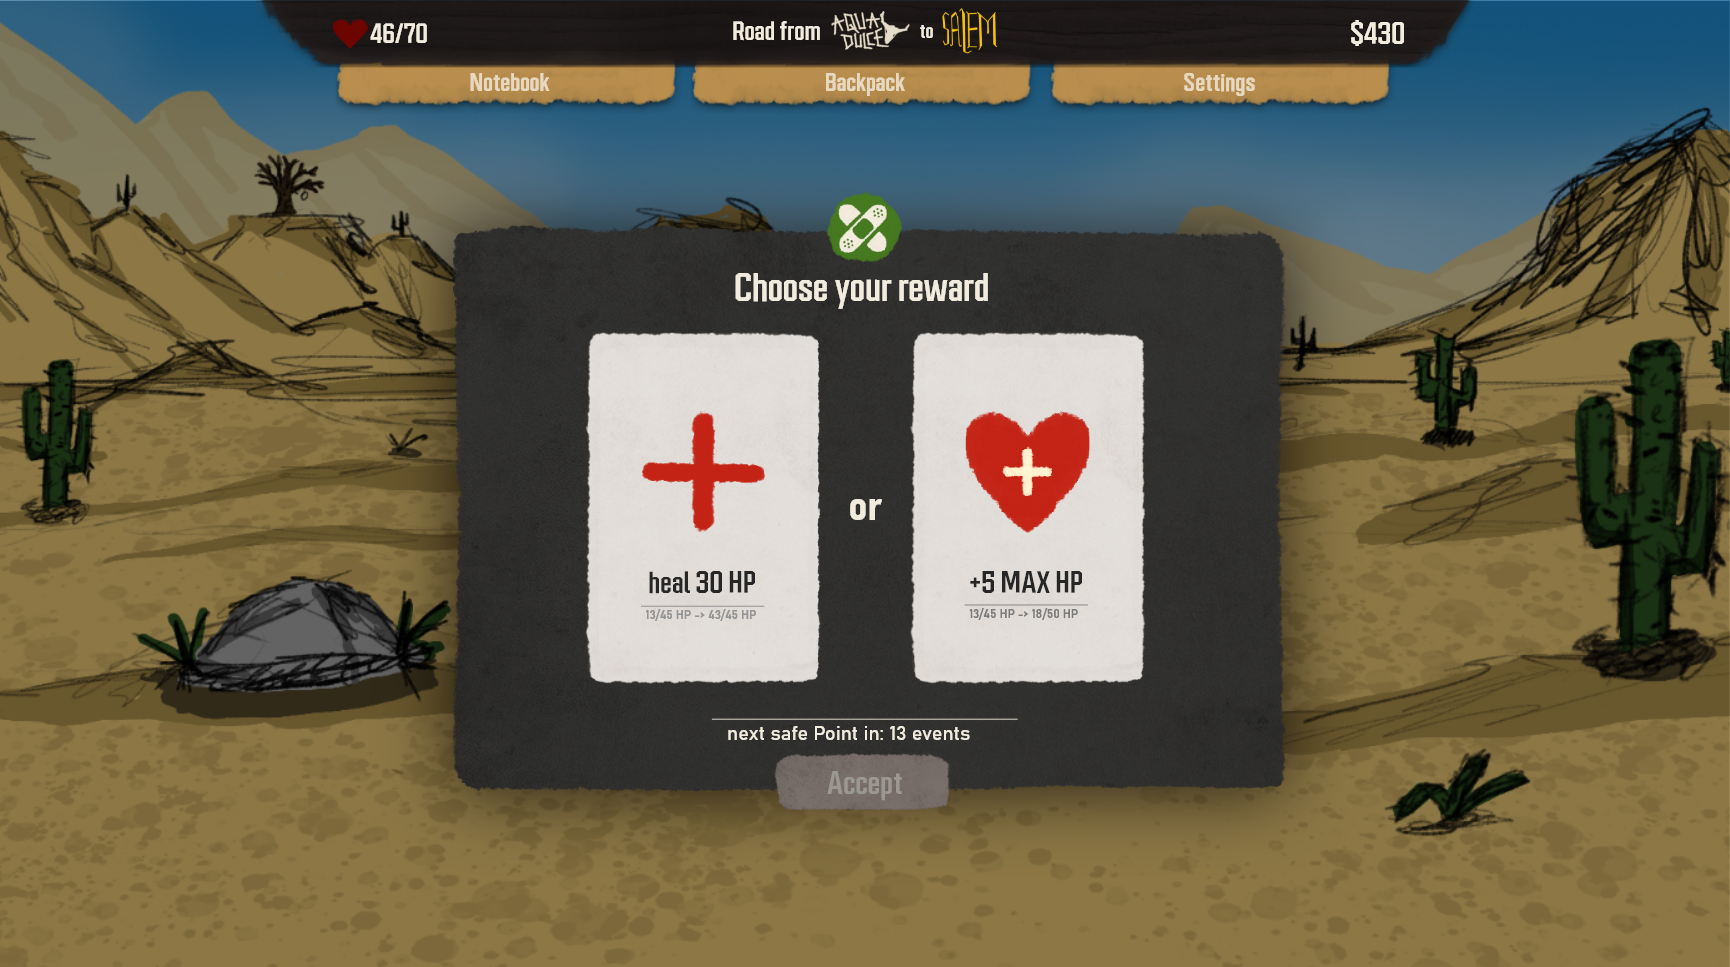
\includegraphics[width=\textwidth]{healeventgrafic.png}
\caption{Beispiel: Ein Heilevent}
\end{figure}


Die zweite Mechanik tritt in Kraft, sollte der Spieler  einen Abschnitt des Spiels, also eine sogenannte Road schaffen. Seine bis zu dem Zeitpunkt gesammelten Karten werden
gespeichert und sind ab dann selbst nach seinem Tod jederzeit zugänglich und spielbar.


Roads werden Abschnitte zwischen zwei Areas genannt und werden zufällig generiert. Areas werden nicht zufällig generiert.

\begin{figure}[H]
    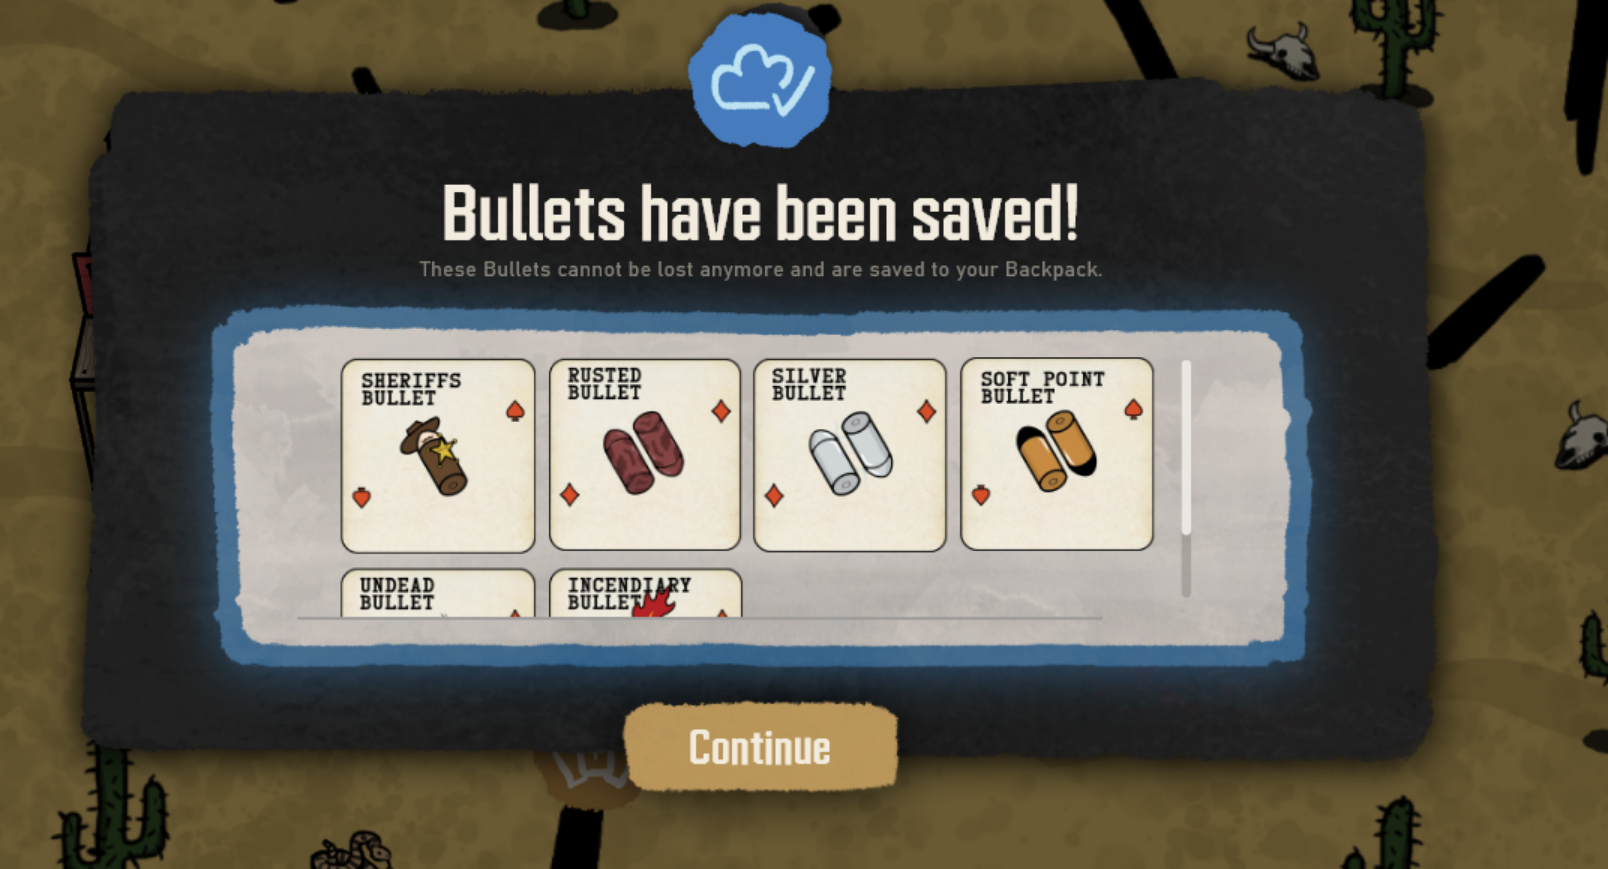
\includegraphics[width=\textwidth]{bulletssavedPopup.png}
    \caption{Beispiel: Das Popup, welches am Ende der Road erscheint um zu zeigen welche Karten gespeichert wurden.}
\end{figure}


\begin{figure}[H]
    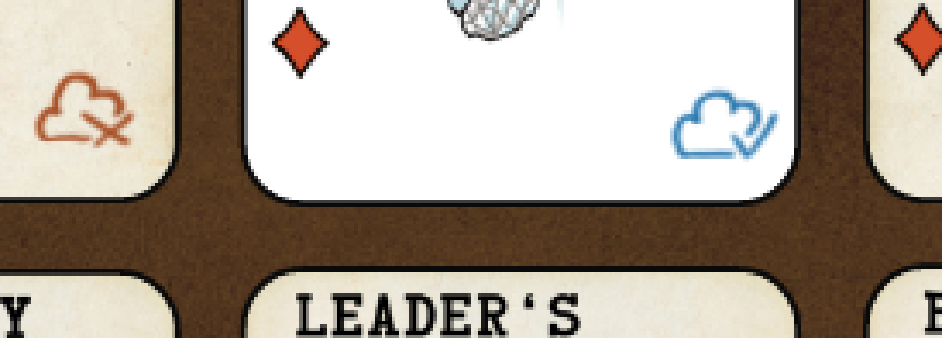
\includegraphics[width=\textwidth]{bulletsaved.png}
    \caption{Beispiel: Symbol einer bereits gespiecherten Karte}
\end{figure}

Verknüpft mit der ersten Mechanik
hat der Spieler die Möglichkeit, sich dazu zu entscheiden, seine Leben wieder aufzufüllen und das Ende der Road anzustreben.
Ist er der Meinung, es sowieso nicht mehr zu dem Abschnittsende zu schaffen, wählt er die Erhöhung der maximalen
Lebenspunkte, um so zumindest einen Vorteil in den nächsten Runs zu haben. Der Spieler muss also das Risiko und die
Belohnung abwägen und dann entscheiden, welche Wahl er trifft.



\subsection{Sammeln von Karten}\label{sammeln_der_Karten}

Nach jedem überlebten Kampf bekommt der Spieler eine neue Karte. Er bekommt drei verschiedene, zufällige Karten presentiert und darf sich eine davon auswählen.
Außerdem gibt es auf der Map verteilt noch zusätzliche Events, die der Spieler aufsuchen kann, um seine Sammlung zu erweitern.

\begin{figure}[H]
    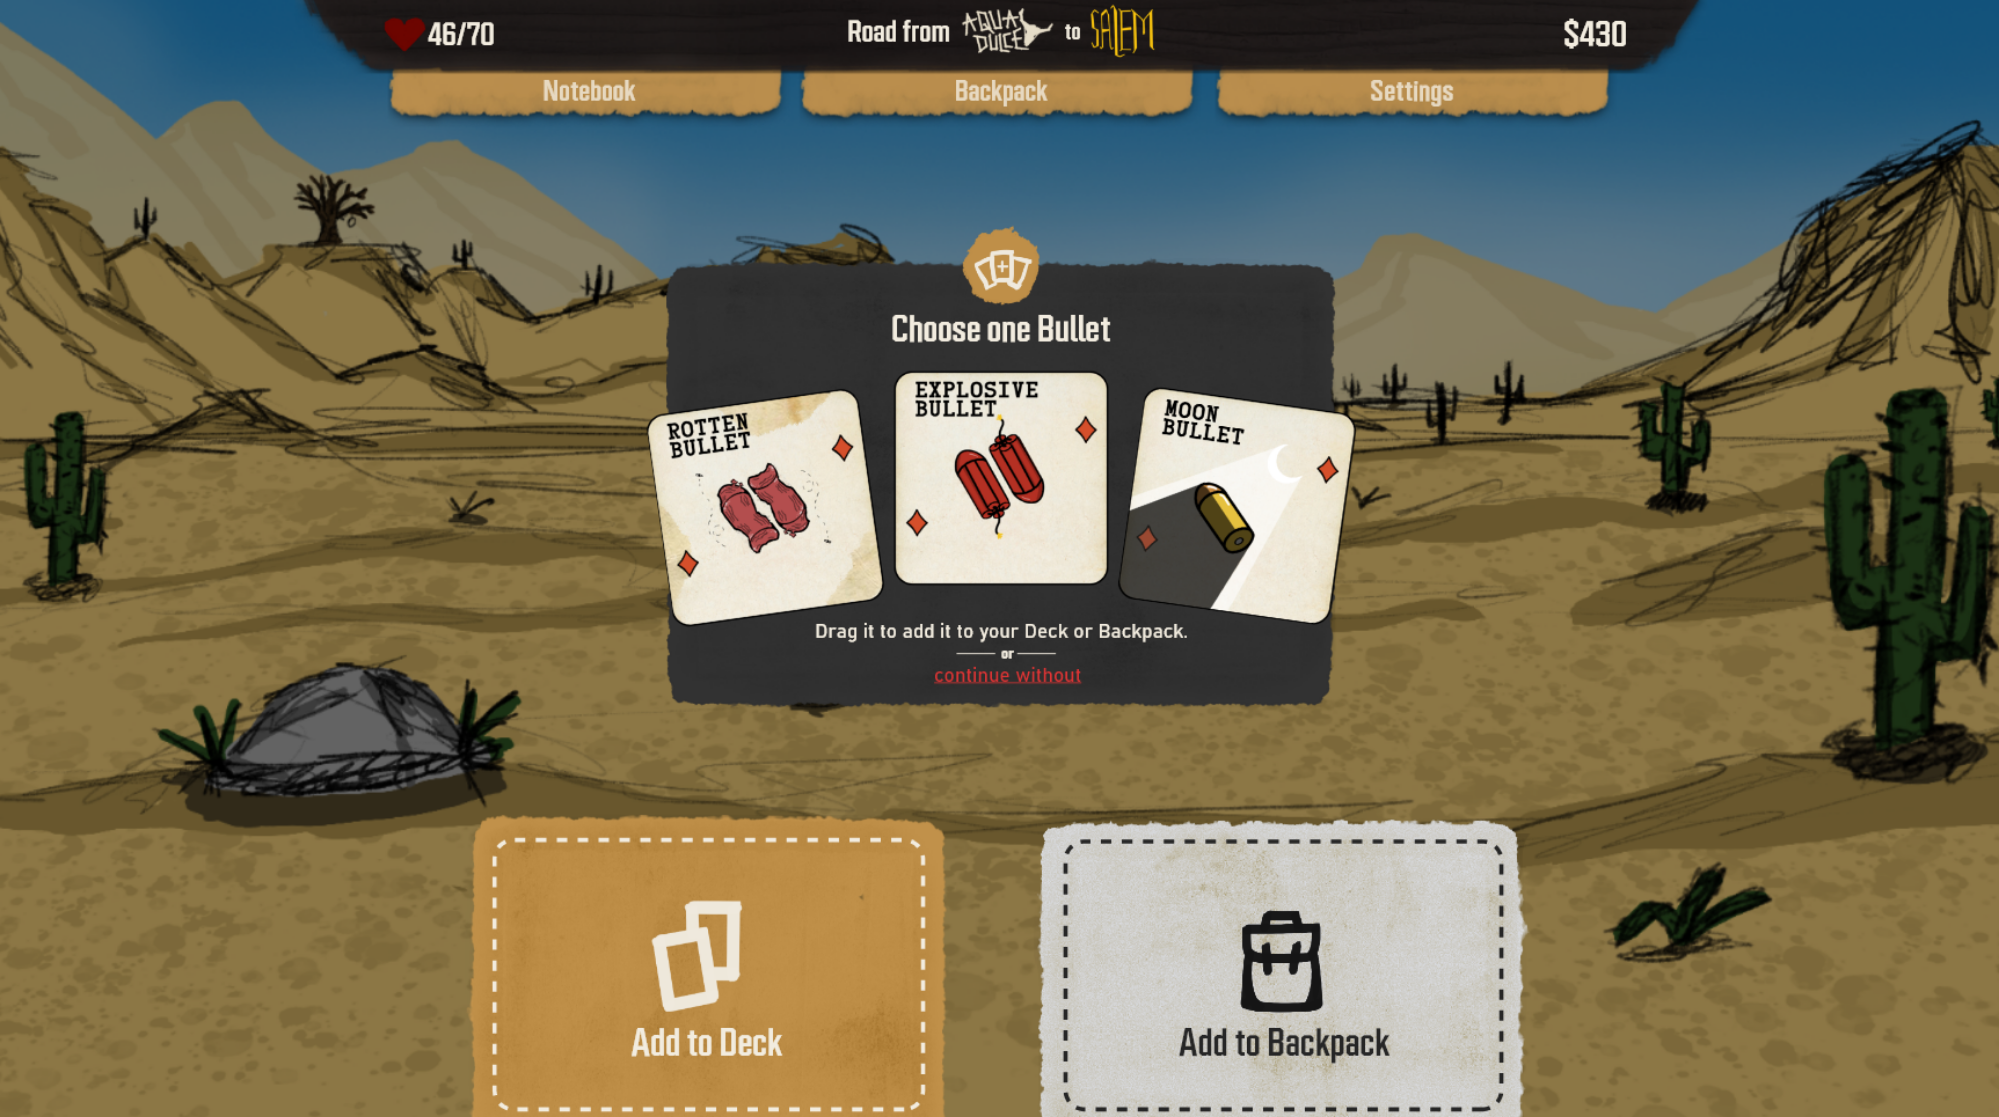
\includegraphics[width=\textwidth]{choosebullet.png}
    \caption{Beispiel: Popup, welches nach einem Kampf, oder auch auf der Map als Event erscheinen kann.}
\end{figure}

Das bringt nicht nur wieder eine Entscheidung des Spielers mit sich, die den Verlauf des Runs ändert, sondern bringt auch mehr Abwechslung,
da der Spieler nicht immer nur die Karten nehmen kann, die er gerne hätte. Es bringt auch eine Art Entdeckerlust mit sich, da der Spieler
auf diese Weise natürlich die Karten erst nach und nach sieht und nicht alle gleich auf einmal, anders als bei \zB "Magic Arena",
wo alle Karten sofort in einer eigenen Liste zugänglich sind. \zit{magicarena} Das zwingt den Spieler mit begrenzter Wahl an Ressourcen das Beste daraus zu machen.

"It is not that players build a deck in order to play the game, it is that they play the game in order to build a deck."\zit{zitatdeckbuilding}%TODO direkte zitate


Diese Designpolitik wird beim Design der Karten beachtet und es wird in dem Kapitel \ref{Gamedesign} näher darauf eingegangen.


Viele Rogue-lite Deckbuilder haben ein ähnliches System. Inspiriert wurde das Sammeln der Karten in \FF von Spielen wie \quoted{Inscription} und \quoted{Slay the Spire},
es gibt jedoch einen großen Unterschied. Anders als in \zB \quoted{Slay the Spire} können Karten ganz einfach aus dem Kartendeck entfernt werden, nachdem sie einmal ausgewählt wurden.
Karten können aus dem Deck in den Backpack verschoben werden und ermöglichen dadurch ein flexibleres Spielerlebnis.\zit{slaythespire, inscryption, zitatdeckbuilding}


\begin{figure}[H]
    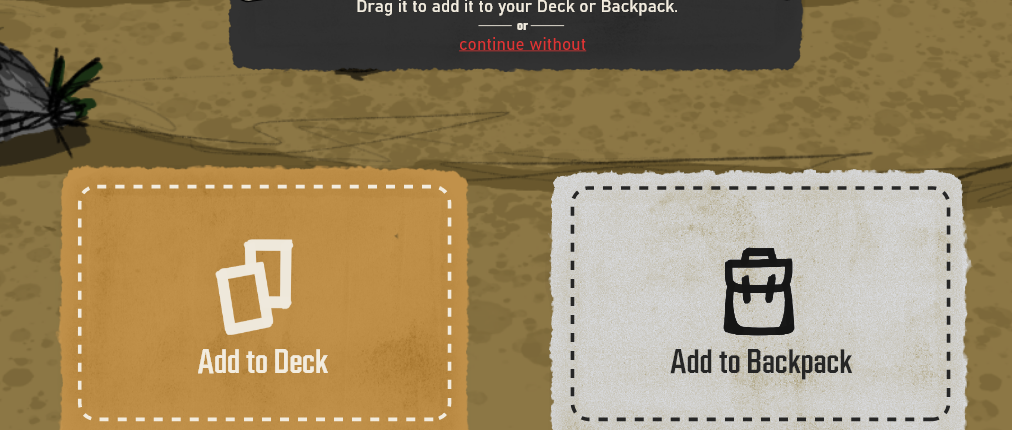
\includegraphics[width=\textwidth]{deckandbackpack.png}
    \caption{Beispiel: zwei Möglichkeiten, nachdem eine Karte ausgewählt wurde}
\end{figure}%

\subsection{Backpack und Deck}\label{backpack_and_deck}

Der Backpack und das Deck dienen beide als Speicherort für Karten, mit dem Unterschied, dass die Karten im Deck aktiv im
Kampf eingesetzt werden und die Karten im Backpack mehr als Reserve gelten.
Karten können frei zwischen den beiden verschoben werden, solange die festgelegte Mindestanzahl an Karten im Deck eingehalten wird.


Da \FF viele verschiedene Strategien bietet, gibt es mehrere Decks, zwischen denen der Spieler einfach wechseln kann.
Das hat zur Folge, dass der Spieler nicht immer ein Deck zerlegen muss, um eine andere Strategie auszutesten.

\begin{figure}[H]
    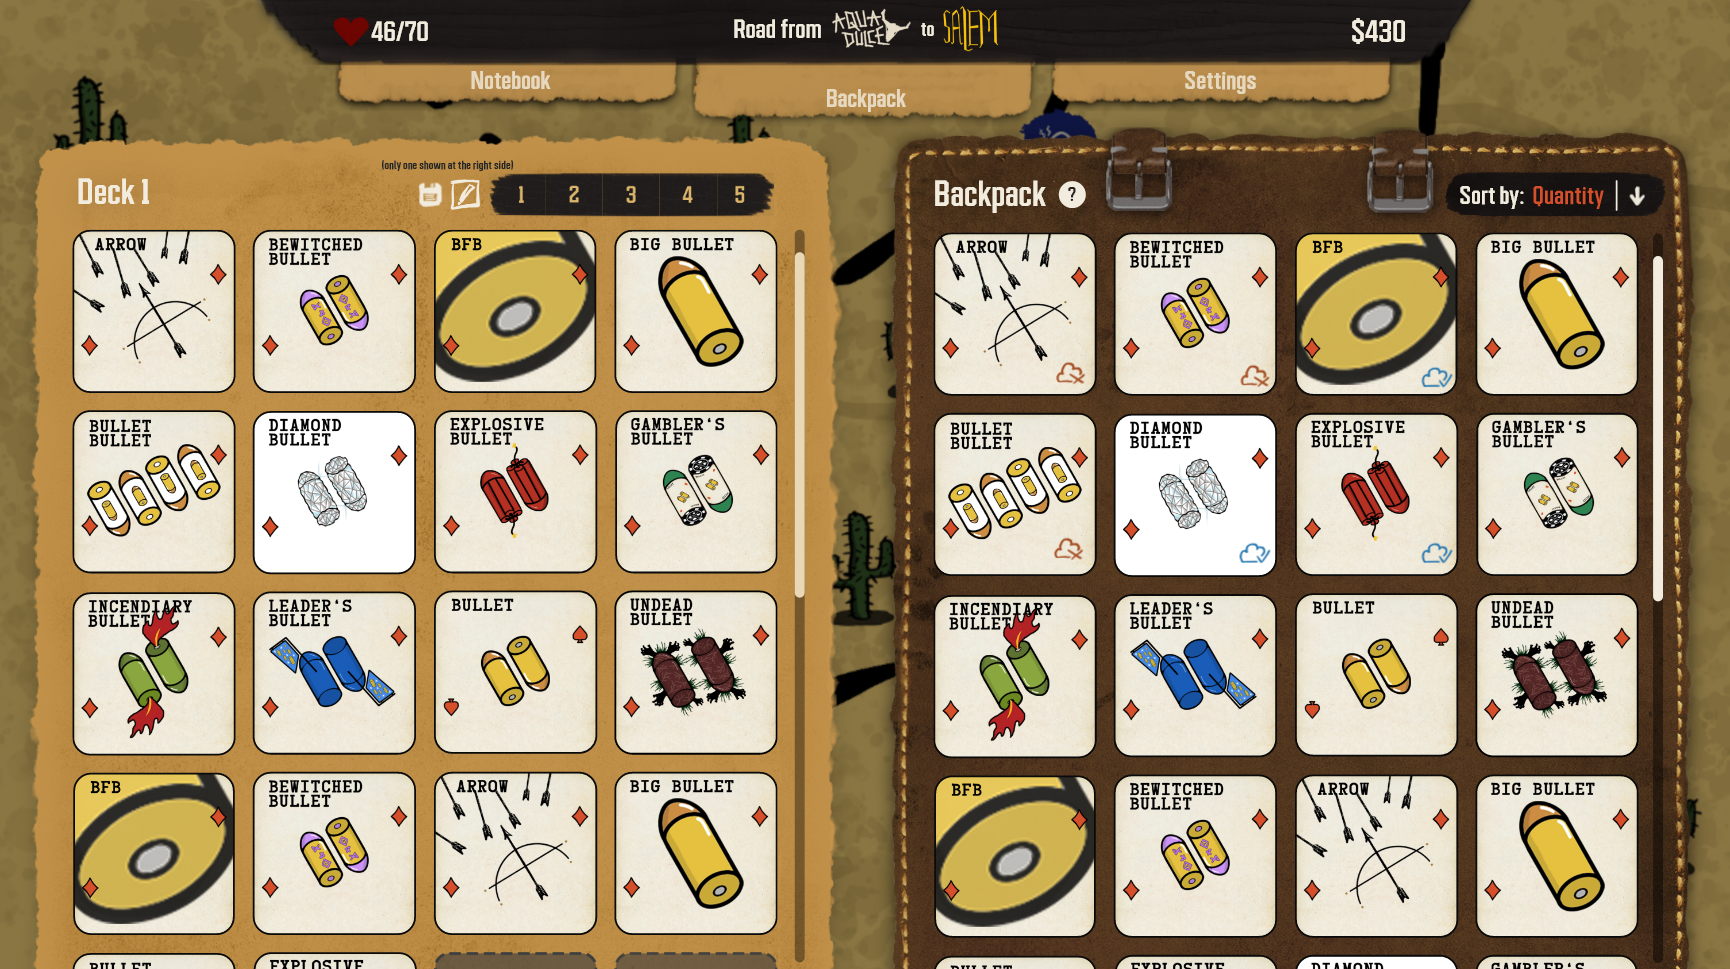
\includegraphics[width=\textwidth]{deckview.png}
    \caption{Beispiel: Ansicht eines Decks und des Backpacks}
\end{figure}

\begin{figure}[H]
    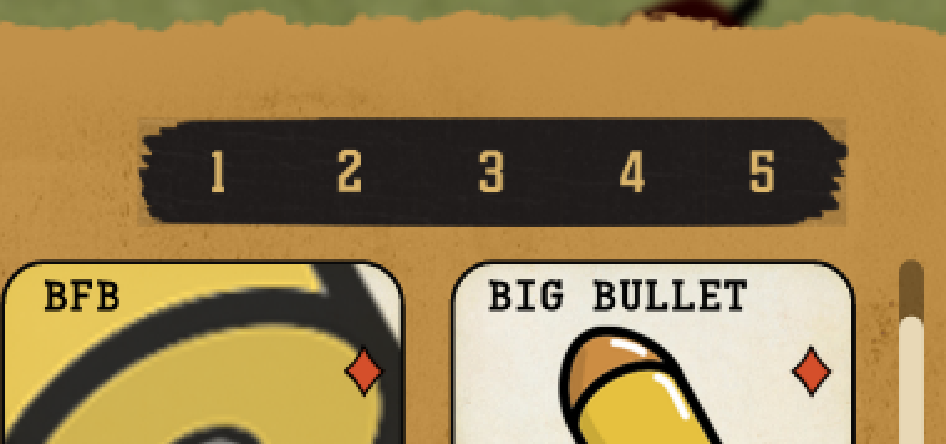
\includegraphics[width=\textwidth]{deckchoose.png}
    \caption{Beispiel: User Interface für das Wechseln des Deckes}
\end{figure}


Außerdem können Decks umbenannt werden, um besser wiedergefunden und erkannt zu werden.

Im Backpack können Karten nach Kriterien wie Kosten oder Namen auf- und absteigend sortiert werden.

\begin{figure}[H]
    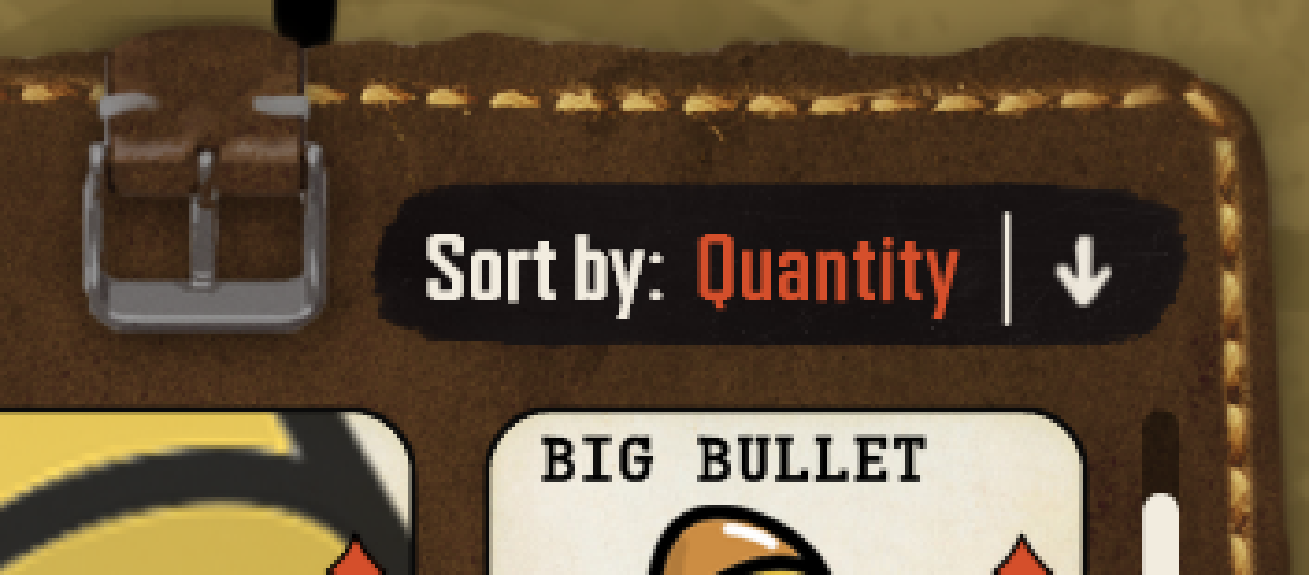
\includegraphics[width=\textwidth]{sortdeck.png}
    \caption{Durch Klicken kann durch verschiedene Sortierungs-Möglichkeiten durchgewechselt werden.}
\end{figure}

Sammelt der Spieler eine neue Karte, kann er sich entscheiden, ob er die Karte gleich seinem Deck oder doch eher seinem
Backpack hinzufügen möchte.
Der Backpack und das Deck ermöglichen es dem Spieler, Karten, die er gesammelt hat, aus dem Deck zu nehmen und damit
nicht zu verwenden, sowie Decks zu bauen, die zu einer Strategie passen.
Startet der Spieler nun einen Kampf, wird das zuletzt ausgewählte Deck verwendet.


\subsection{Kampf}\label{backpack_and_deck}
%grundsätzliche sachen wie reserves, gegner und spieler, gewonnen wenn gegner tod usw karten am anfang ziehe zwei karten am anfang vom turn

Während der Spieler über die Map reist, sind Kämpfe unausweichlich.


Kämpfe werden auf der Map durch zwei gekreuzte Revolver dargestellt. Um weiter auf der Map fortzuschreiten müssen sie absolviert werden.

\begin{figure}[H]
    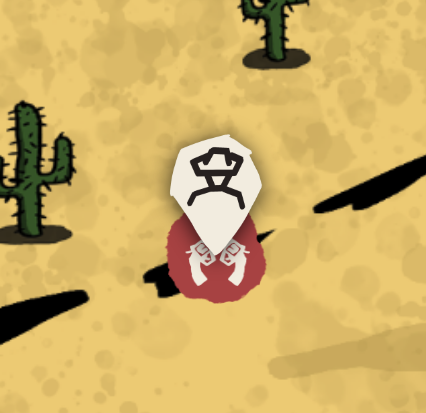
\includegraphics[width=\textwidth]{playericon.png}
    \caption{Beispiel: Eventsymbol für einen Kampf}
\end{figure}

Gekämpft wird mit den gesammelten Karten, mit dem Ziel, den oder die Gegner zu besiegen und dabei so wenig Lebenspunkte
wie möglich zu verlieren \bzw nicht zu sterben.

Gewonnen hat der Spieler, wenn alle Gegner besiegt wurden.


Ein Kampf ist aufgeteilt in Züge. Immer abwechselnd ist entweder der Spieler oder der Gegner dran. Am Anfang des Kampfes
werden eine vordefinierte Anzahl an Karten vom Deck des Spielers gezogen.
Anschließend hat der Spieler die Möglichkeit, nach Belieben seinen Zug auszuführen. Ein Spielerzug wird mit dem "Holster"
Button beendet, und das Betätigen des Knopfes startet den automatischen Ablauf des Gegnerzuges. Der Gegner führt eine -mehr
oder weniger- zufällige Aktion aus, und danach ist wieder der Zug des Spielers.


Am Start des Zuges des Spielers werden zwei Karten vom Deck gezogen. Pro Zug stehen dem Spieler vier "Reserves"
zur Verfügung. Diese werden jeweils auch am Anfang des Zuges wieder auf die maximale Anzahl aufgefüllt.
Reserves können dazu verwendet werden, Karten zu bezahlen und damit auch zu spielen.

\begin{figure}[H]
    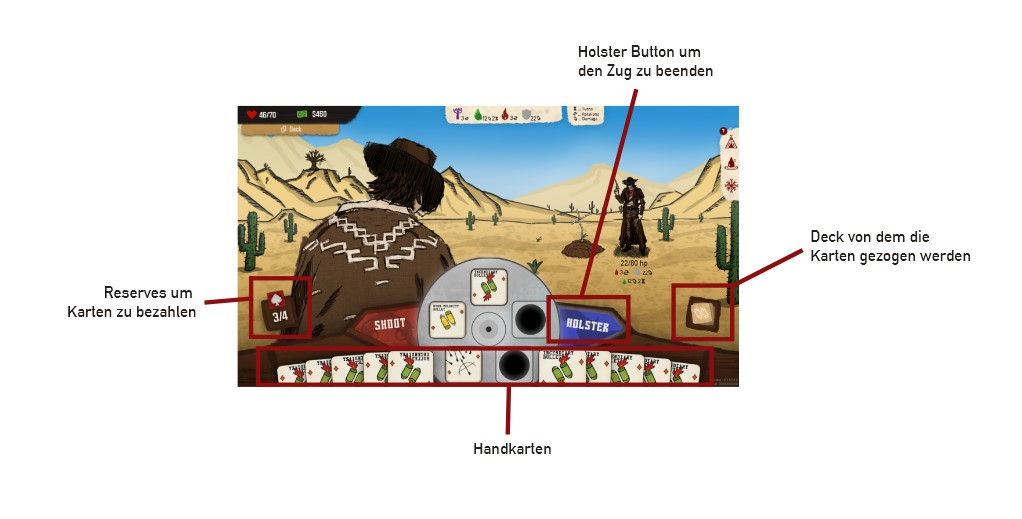
\includegraphics[width=\textwidth]{turngrafic.jpg}
    \caption{Beispiel: Kampf User-Interface in welchem alle benötigten Infos dargestellt werden.}
\end{figure}



\subsection{Karten}\label{Karten}
Karten in \FF sind Bullets. Jede Bullet hat einen Kosten-Wert, der mit "Reserves" bezahlt werden muss, um die Karte zu spielen, also zu benützen.
Die "Reserves", die für die Bullet benötigt werden, werden automatisch bezahlt, falls der Spieler sich die Bullet leisten kann.
Ein gutes Management der Reserves und die Reihenfolge, in der man die Karten spielt, ist wichtig, um das Spiel zu meistern.


Jede Bullet hat außerdem einen Damage-Wert, auch Schadens-Wert, Dmg-Value oder Dmg-Wert genannt, welcher angibt, wie viele Lebenspunkte dem Gegner
durch die Karte abgezogen werden, falls die Karte auf den Gegner geschossen wird.

\begin{figure}[H]
    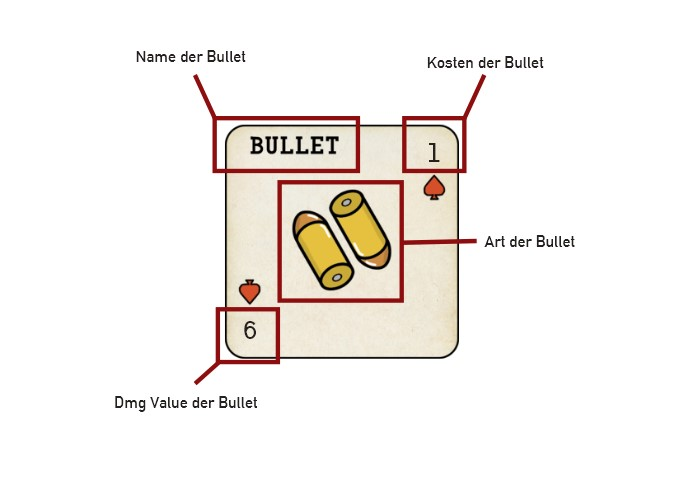
\includegraphics[width=\textwidth]{bulletgrafic.jpg}%TODO BILD ändern bullet grafik
    \caption{Beispiel: Die wichtigsten Infos werden auf der Karte angezeigt.}
\end{figure}

Fast alle Karten haben außerdem einen einzigartigen Effekt,
welcher angesehen werden kann, indem der Spieler mit der Maus über die gewünschte Bullet hovert.
In dem Popup, welches nach dem Hovern sichtbar ist, befinden sich die Infos zu dem Effekt der Karte.
Dazu gehört fast immer ein Trigger und der Effekt selbst.


Der Trigger gibt an, wann sich der Effekt aktiviert.


\begin{figure}[H]
    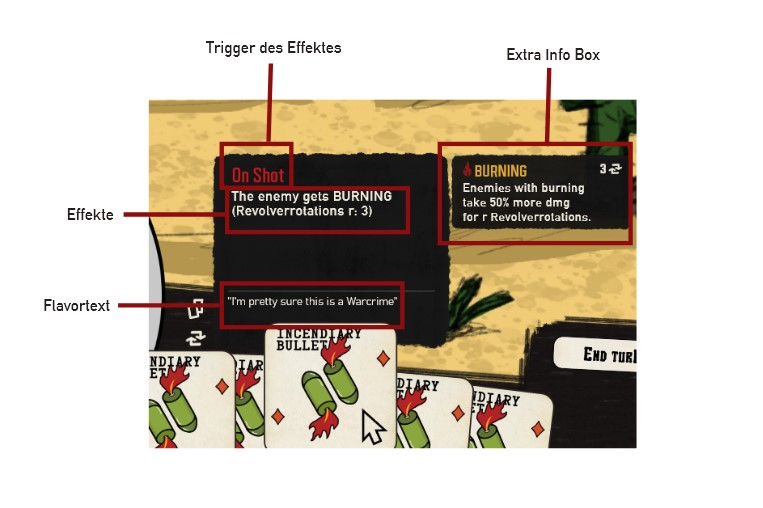
\includegraphics[width=\textwidth]{hovergrafic.jpg}
    \caption{Beispiel: Hoverdetails,welche Infos über die karte zeigen}
\end{figure}



Es gibt verschiedene Trigger, wie \zB das Aktivieren des Effektes beim Spielen der Bullet.


Zusätzlich zu dem Effekt und dem Trigger steht bei vielen Karten außerdem noch ein Flavortext.
Ein Flavortext ist ein Spruch, der der Bullet ein wenig Kontext hinzufügt.
Es kann sich um einen Spruch, einen Witz, eine Anspielung oder einen story- \bzw worldbuilding-relevanten Text handeln.


Falls nötig werden relevante Infos zu dem Effekt in einer extra Box rechts oder links angezeigt.


Bullets werden, wenn sie gespielt werden, in den Revolver geladen.


\subsection{Revolver}\label{der_revolver}

Der Revolver ist das Spielfeld von \FF, in welches die Bullets platziert \bzw "geladen" werden.
Mithilfe von "Drag and Drop" kann der Spieler die Karte aus seiner Hand in den Revolver legen, diese Aktion des Ladens wird auch als Spielen der Bullet bezeichnet.
Im Zug des Vorganges werden Reserves in Höhe des Kosten-Wertes der Bullet abgezogen.


Der Revolver besteht aus fünf Kammern bzw. Feldern, in die Bullets geladen werden können.
Sie sind intern von eins bis fünf nummeriert.


Der Revolver kann von dem Spieler abgefeuert werden. Wenn geschossen wird, wird die Bullet in der obersten Kammer auf den Gegner geschossen.
Verlässt sie den Revolver, verliert der Gegner Lebenspunkte in Höhe des Damage-Wertes der geschossenen Bullet.
Die Bullet wird unter das Deck gelegt und der Revolver dreht sich einmal nach rechts.

\begin{figure}[H]
    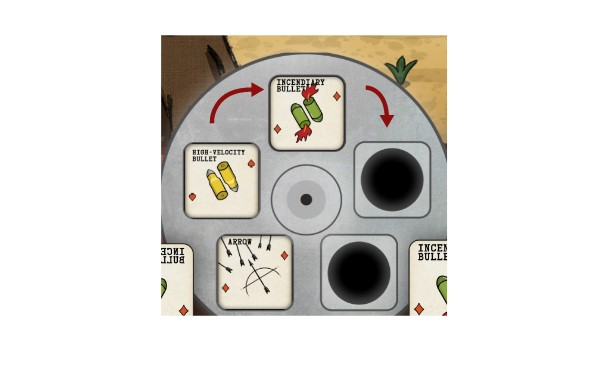
\includegraphics[width=\textwidth]{rotategrafic.jpg}
    \caption{Beispiel: Revolverdrehung nach rechts}
\end{figure}


Die Revolverrotation ist ein wichtiger Teil von \FF, da der Spieler sich das Placement der Bullets im Revolver genau überlegen muss,
um das Meiste aus seinen Bullets herauszuholen.


Weiters gibt es Karten mit Effekten, die sich auf die Revolverrotation auswirken, wie \zB "Bewitched Bullet",
welche den Revolver nach links statt nach rechts rotiert.


Die Komplexität von \FF kommt vom Meistern des Revolvers, der strategischen Platzierung und Reihenfolge der Bullets und dem Verstehen,
wie eine Revolverrotation sich auf die Bullets, den Spieler oder den Gegner auswirkt.


Die "Bewitched Bullet" kann \zB dazu verwendet werden, Karten,
welche davon profitieren, lange im Revolver zu bleiben, länger vom Abschuss zu bewahren. "Bull et" zum Beispiel fügt dem Gegner Schaden zu,
wenn sie im Revolver rotiert und profitiert damit von der Linksdrehung von Bewitched Bullet.


\begin{figure}[H]
    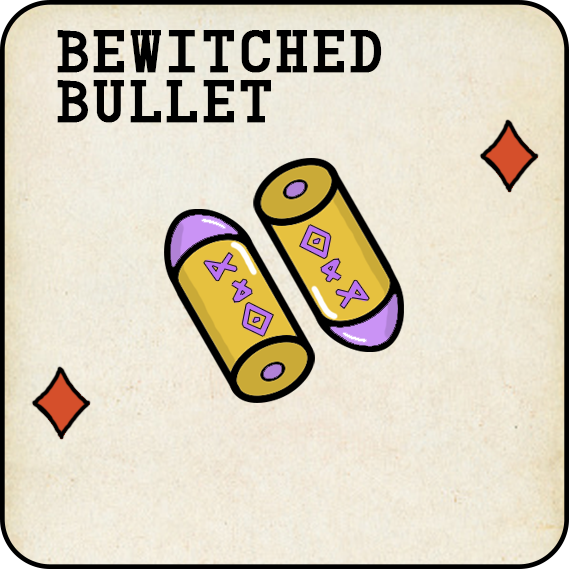
\includegraphics[width=50\%]{bewitched_Bullet.png}
    \caption{Beispiel: Bewitched Bullet}
\end{figure}

\begin{figure}[H]
    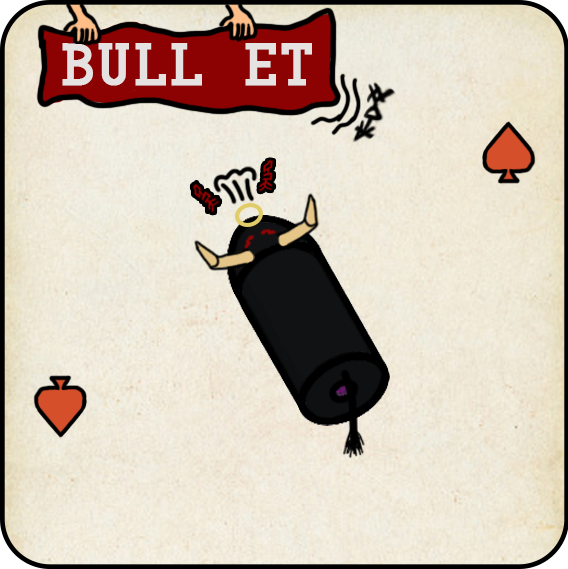
\includegraphics[width=50\%]{bull_et.png}
    \caption{Beispiel: Bewitched Bullet}
\end{figure}


\subsection{Gegner}\label{gegner}
Der Gegner, auf den die Bullets des Spielers geschossen werden, besteht aus mehreren Komponenten.
Genau wie der Spieler verfügt der Gegner über einen HP-Wert. Wenn der Wert null erreicht, stirbt der Gegner.


Während dem Zug des Spielers zeigt der Gegner die Aktion an, die er in seinem nächsten Zug ausführen wird.
Nachdem der Spieler "Holster" gedrückt hat, beendet er seinen Zug und der Gegner ist dran.

Gegneraktionen werden zufällig ausgewählt aus dem Pool von Aktionen.
Jedoch wurden die Aktionen angepasst, um nicht nur Fairness zu garantieren,
sondern auch eine Balance zwischen mehr oder weniger anspruchsvoll zu finden.
Mehr zum Balancen der Gegner kann im Kapitel \ref{Gamedesign} nachgelesen werden.


Sobald der Gegner am Zug ist, wird die Aktion automatisch ausgeführt. Je nach Gegnertyp gibt es andere Aktionen,
die ein Gegner ausführen kann. Universell ist jedoch die Aktion des Schaden zufügens.
Es gibt viele verschiedene Arten von Gegneraktionen, die dafür entwickelt wurden, mehr Abwechslung beim Bekämpfen der Gegner zu bieten.

Das Gegnerverhalten ist entstanden durch das Beobachten von Spielen im selben Genre, wie zum Beispiel \quoted{Slay the Spire}. \zit{slaythespire}


Außerdem sollte noch erwähnt werden, dass es auch passieren kann, dass der Spieler gegen mehr als einen Gegner kämpft.
Ist das der Fall, markiert der Spieler sein Ziel, indem er auf den gewünschten Gegner klickt.



Die geplannten Aktionen der Gegner sind durch Symbole über ihren Köpfen dargestellt. Der spieler hat die Aufgabe,
diese Aktionen in die Plannung seines Zuges miteinzubeziehen. Eine mögliche Reaktion auf das Zufügen von Schaden ist das parrieren.


\subsection{Parrying}\label{parrying}
Das parieren des Schadens, der vom Gegner verursacht wird, wird in \FF durch Bullets erreicht.


Der Spieler bekommt die Wahl, ob er parieren möchte oder nicht, was durch ein eigenes Popup während des gegnerischen Zuges geregelt wird.
Entscheidet sich der Spieler dazu zu parieren, wird dafür die Bullet im vordersten Slot verwendet.
Dann wird der Schadenswert des Gegners mit dem der Bullet gegengerechnet. Ist der Schadenswert der Bullet größer als der des Gegners,
geht kein Schaden durch. Ist es andersrum, bekommt der Spieler so viel Schaden zugefügt wie die Differenz ausmacht.


Es ist wichtig zu erwähnen, dass nicht pariert werden muss, wenn der Spieler die Bullet lieber behalten will, und den Schaden einfach einzustecken kann.
Durch einen Parry verlässt die Bullet den revolver und sie wird danach wieder unters Deck gelegt.


\subsection{Spezifische Regeln}\label{spezifische_regeln}

Es gibt einige zusätzliche spezifische Regeln in \FF. Beispielhaft werden folgende zwei erläutert.

\subsection{Overkillschaden}\label{Overkill}

Die erste ist der sogenannte Overkillschaden.
Die Regel besagt, dass jeglicher Schaden, der dem Gegner zugefügt wird, nachdem seine Lebenspunkte bereits unter 0 sind,
in Geld umgewandelt wird. Das Geld kann benutzt werden, um sich bei einem Shop weitere Karten zu kaufen.
Die Overkill-Regel gilt jedoch nur für den aktuellen Zug. Drückt der Spieler auf "Holster", wird der Zug und der Kampf beendet.


Overkill-Cash, das durch Overkillschaden verdiente Geld, ist nicht nur eine gute Möglichkeit, Belohnungen anhand der Leistung des Spielers zu berechnen.


sondern löst auch gleichzeitig folgendes Problem: In \FF ist der Aufbau des Revolvers und damit von Combos sehr wichtig.
Oft kommt es vor, dass der Spieler eine Combo aufgebaut hat, der Gegner jedoch einfach schneller tot ist.
Das ist nicht nur frustrierend, sondern gibt dem Spieler auch einfach keinen Grund, überhaupt starke Combos aufzubauen,
wenn er sich einmal über dem Standard-Gegner-Schwierigkeitslevel befindet. Overkill-Schaden löst diese beiden Probleme.


\subsection{Leerschüsse}\label{leerschüsse}

Die zweite Regel bezieht sich auf das Schießen des Revolvers.
Die Regel besagt, dass, wenn der Revolver leer geschossen wird, also keine Bullet in der vordersten Kammer vorhanden ist,
der Spieler 5 Lebenspunkte Schaden erleidet.

Die örtliche Platzierung, der Zeitpunkt und die reihenfolge ist das wichtigste beim Platzieren der Bullets.

Einen Bullet in den hintersten oder ersten Slot zu platzieren, ist eine Entscheidung, die überlegt sein sollte.
Ohne die Leerschuss-regel ist es jedoch möglich, Bullets, die man weiter hinten platziert hat, sofort wieder vorrotieren zu lassen,
was das gesamte Spielprinzip der Revolverrotation ruinieren würde, da das Platzieren keine Konsequenzen hätte.
Es würde dazu führen, dass Bullets nacheinander einfach in den Revolver geladen werden, wo es gerade passt, und sofort
geschossen werden, da die Schussreihenfolge der Bullets ja sowieso egal ist.


Jedoch wollten die Entwickler das Rotieren des Revolvers ohne eine Bullet in dem vordersten Slot durch das Schießen nicht verbieten, sondern führten ein,
dass 5 Lebenspunkte abgezogen werden. Das bedeutet also, dass es im Notfall gemacht werden kann, z.B. falls es einmal für
eine Combo nötig ist, jedoch nicht durchgehend benutzt werden kann, da der Spieler durch das Abziehen der Lebenspunkte sonst stirbt.
Es ist eigentlich ein perfektes Beispiel, wie man durch das nicht direkte Verbieten einer Mechanik die Komplexität und
Möglichkeitsvielfalt wachsen lassen kann.


\subsection{Encounter Modifier}\label{encounter_modifier}


Encounter Modifier sind extra Regeln, die einem Kampf hinzugefügt werden um noch mehr Abwechslung in das Spiel zu bringen
und um den Spieler auch manchmal zum Wechseln der Kartenstrategien zu bringen.
Sie sind vor dem Kampf einsehbar, um das Umbauen oder Wechseln eines Decks noch zu ermöglichen.
Encounter Modifier können ganz verschieden sein.

Es gibt verschiedene Arten von Modifiern, einige untertützen, andere Schaden dem Spieler. Andere wiederum stellen die Regeln von \FF auf den Kopf.
Der Encounter Modifier "Frost" zum Beispiel friert den Revolver ein, was die Auswirkung hat, dass sich der Revolver  nach einem Schuss nicht mehr dreht.
"Bewitched Mist" lässt den Revolver immer statt nach rechts nach links drehen, was natürlich auch sehr verwirrend sein kann.

% resets author
\renewcommand{\kapitelautor}{}
